%%%%%%%%%%%%%%%%%%%%%%%%%%%%%%%%%%%%%%%%%
% Beamer Presentation
% LaTeX Template
% Version 1.0 (10/11/12)
%
% This template has been downloaded from:
% http://www.LaTeXTemplates.com
%
% License:
% CC BY-NC-SA 3.0 (http://creativecommons.org/licenses/by-nc-sa/3.0/)
%
%%%%%%%%%%%%%%%%%%%%%%%%%%%%%%%%%%%%%%%%%

%----------------------------------------------------------------------------------------
%	PACKAGES AND THEMES
%----------------------------------------------------------------------------------------

\documentclass{beamer}

\mode<presentation> {

% The Beamer class comes with a number of default slide themes
% which change the colors and layouts of slides. Below this is a list
% of all the themes, uncomment each in turn to see what they look like.

%\usetheme{default}
%\usetheme{AnnArbor}
%\usetheme{Antibes}
%\usetheme{Bergen}
%\usetheme{Berkeley}
%\usetheme{Berlin}
%\usetheme{Boadilla}
%\usetheme{CambridgeUS}
%\usetheme{Copenhagen}
%\usetheme{Darmstadt}
%\usetheme{Dresden}
%\usetheme{Frankfurt}
%\usetheme{Goettingen}
%\usetheme{Hannover}
%\usetheme{Ilmenau}
%\usetheme{JuanLesPins}
%\usetheme{Luebeck}
\usetheme{Madrid}
%\usetheme{Malmoe}
%\usetheme{Marburg}
%\usetheme{Montpellier}
%\usetheme{PaloAlto}
%\usetheme{Pittsburgh}
%\usetheme{Rochester}
%\usetheme{Singapore}
%\usetheme{Szeged}
%\usetheme{Warsaw}

% As well as themes, the Beamer class has a number of color themes
% for any slide theme. Uncomment each of these in turn to see how it
% changes the colors of your current slide theme.

%\usecolortheme{albatross}
%\usecolortheme{beaver}
%\usecolortheme{beetle}
%\usecolortheme{crane}
%\usecolortheme{dolphin}
%\usecolortheme{dove}
%\usecolortheme{fly}
%\usecolortheme{lily}
%\usecolortheme{orchid}
%\usecolortheme{rose}
%\usecolortheme{seagull}
%\usecolortheme{seahorse}
%\usecolortheme{whale}
%\usecolortheme{wolverine}

%\setbeamertemplate{footline} % To remove the footer line in all slides uncomment this line
%\setbeamertemplate{footline}[page number] % To replace the footer line in all slides with a simple slide count uncomment this line

%\setbeamertemplate{navigation symbols}{} % To remove the navigation symbols from the bottom of all slides uncomment this line
}

\usepackage{graphicx} % Allows including images
\usepackage{booktabs} % Allows the use of \toprule, \midrule and \bottomrule in tables

%----------------------------------------------------------------------------------------
%	TITLE PAGE
%----------------------------------------------------------------------------------------

\title[]{Problems 3.17} % The short title appears at the bottom of every slide, the full title is only on the title page

\author{Jatoth Vishwajith Rathod} % Your name
\institute[] % Your institution as it will appear on the bottom of every slide, may be shorthand to save space
{
IIT Hyderabad \\ % Your institution for the title page
\medskip
\textit{ee16btech11014@iith.ac.in} % Your email address 
}
\date{\today} % Date, can be changed to a custom date

\begin{document}

\begin{frame}
\titlepage % Print the title page as the first slide
\end{frame}



%----------------------------------------------------------------------------------------
%	PRESENTATION SLIDES
%----------------------------------------------------------------------------------------

%------------------------------------------------


\begin{frame}
\frametitle{Question 3.17}
\begin{equation*}
     \min_{x} \textbf{x1 + x2}
\end{equation*}
With constraints\\

\begin{center}
 x_1^2 - x_1 + x_2^2  \leq 0$\\
 where x = \begin{pmatrix}
    x_1  \\
    x_2  \\
   \end{pmatrix} 
\end{center}

\end{frame}




%------------------------------------------------

\begin{frame}
\frametitle{Solution}
Using the method of Lagrangian multipliers,

\begin{center}
\begin{equation*}
\nabla{ f(x) + \mu g(x)} =0  ,    \mu \geq 0$\\

resulting in the equations\\
2x_1\mu - \mu + 1 = 0 \\
2x_2\mu + 1 = 0 \\
x^2_1 - x_1 + x^2_2 = 0 \\
\end{equation*}
\end{center}


\end{frame}


%------------------------------------------------



%------------------------------------------------

\begin{frame}
\frametitle{Solution}

\begin{equation*}
\begin{center}
        which can be simplified to obtain 
%
\begin{align}
\brak{\frac{1-\mu}{2\mu}}^2 + \brak{\frac{1}{2\mu}}^2 + \frac{1-\mu}{2\mu} &= 0 \\
\Rightarrow 1 + \mu^2 -2\mu + 1 + 2\mu\brak{1-\mu} &= 0 \\
\Rightarrow \mu^2 =2, or \mu &= \pm \sqrt{2} 
\end{align}
%

 $\mu \ge 0 \Rightarrow  \mu = \sqrt{2}$.

\end{center} 
\end{center}
\end{frame}

%----------------------------------------------------------------------------------------
\begin{frame}{Solution}

The desired solution is
%
\begin{equation}
\mbf{x} = 
\begin{pmatrix}
 \frac{\sqrt{2}-1}{2\sqrt{2}} \\
-\frac{1}{2\sqrt{2}} 
\end{pmatrix}
\end{equation}
%
{\em Graphical solution:} The constraint can be expressed as
%
\begin{align}
x_1^2 - x_1 + x_2^2 &\le 0 \\
\Rightarrow \brak{x_1 - \frac{1}{2}}^2 + x_2^2 & \le \brak{\frac{1}{2}}^2
\end{align}
%
\end{frame}




\begin{frame}{Solution}

\begin{figure}[!ht]
\centering
\includegraphics[width=\columnwidth]{./figs/2.15.eps}
\caption{ Optimal solution is the lower tangent to the circle}
\label{fig.2.15}	
\end{figure}
%

\end{frame}


\begin{frame}{Solution}
\begin{center}
    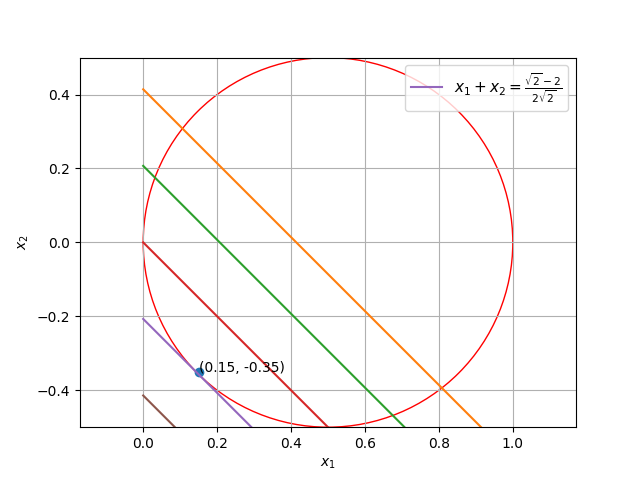
\includegraphics[scale=0.5]{Figure_1.png}
\end{center}
\end{frame}

\begin{frame}{And last}
\begin{center}
    Thank You
\end{center}
\end{frame}
\end{document} 